\chapter{Security Considerations}
\label{cha:Security}

In this chapter we are going to discuss in more details the cryptographic principles that ensure security. Firstly we are going to analyze X3DH and later the double ratchet mechanism. But before starting we need to define some preliminaries used in each of the two algorithms.

\section{Preliminaries}
\label{sec:Preliminaries}

As explained above an application using X3DH must decide on several parameters:

\vspace{0.5cm}
\begin{center}
\begin{tabular}{>{\itshape}l p{10cm}}
\toprule
Name & Definition \\
\midrule
curve & X25519 or X448 \\
hash & A 256 or 512-bit hash function (e.g. SHA-256 or SHA-512) \\
info & An ASCII string identifying the application \\
\bottomrule
\end{tabular}
\end{center}

\vspace{0.5cm}

In our protocol we used \textbf{X25519}, as hash \textbf{SHA}. An application must additionally define an encoding function Encode(PK) to encode an X25519 or X448 public key PK into a byte sequence. Since we decided to implement only one of the two curves there was no need to differentiate between them.

\section{Cryptographic Notation}
\label{sec:Crytpographic Notation}

The used notation in this chapter is:

\begin{itemize}
  \item The concatenation of byte sequences \textbf{X} and \textbf{Y} is $\textbf{X} \| \textbf{Y}$
  \item $\textbf{DH(PK1,PK2)}$ represents a byte sequence which is the shared secret output from an Elliptic Curve Diffie-Hellman function involving the key pairs represented by public keys $PK1$ and $PK2$. The Elliptic Curve Diffie-Hellman function will be the $X25519$.
  \item $\textbf{Sig(PK,M)}$ represents a byte sequence that is an \textbf{XEdDSA} signature on the byte sequence $M$ and verifies with public key $PK$, and which was created by signing $M$ with $PK$'s corresponding private key.
  \item \textbf{KDF(KM)} represents 32 bytes of output from the $HKDF$ algorithm with inputs:
  \begin{itemize}
    \item $HKDF$ $input$ $key$ $material = F \| KM$, where $KM$ is an input byte sequence containing secret key material, and $F$ is a byte sequence containing $32$ $0xFF$. $F$ is used for cryptographic domain separation with $XEdDSA$.
    \item $HKDF$ $salt =$ a zero-filled byte sequence with length equal to the $hash$ output length.
    \item $HKDF$ $info =$ the $info$ parameter.
  \end{itemize}
\end{itemize}

\section{Roles}
\label{sec:Roles}

The X3DH protocol involves theree parties: \textbf{Alice, Bob} and a \textbf{server}.

\begin{itemize}
  \item \textbf{Alice} wants to send to Bob some initial data using encryption, and also establish a shared secret key.
  \item \textbf{Bob} wants to allow parties like Alice to establish a shared key with him and send encrypted data. However, Bob might be offline when Alice attempts to do this. To enable this, Bob has a relationship with some server.
  \item \textbf{The server} can store messages from Alice to Bob which Bob can later retrieve. The server also lets Bob publish some data which the server will provide to parties like Alice.
\end{itemize}

\section{Keys}
\label{sec:Keys}

X3DH used the following elliptic curve keys:

\begin{center}
\begin{tabular}{>{\itshape}l l}
\toprule
Name & Definition \\
\midrule
$IK_A$ & Alice’s identity key \\
$EK_A$ & Alice’s ephemeral key \\
$IK_B$ & Bob’s identity key \\
$SPK_B$ & Bob’s signed prekey \\
$OPK_B$ & Bob’s one-time prekey \\
\bottomrule
\end{tabular}
\end{center}

All public keys have a corresponding private key, but to simplify description we will focus on the public keys. Each party has a long-term identity public key ($IK_A$ for Alice, $IK_B$ for Bob). Bob also has a signed prekey $SPK_B$, which he will change periodically, and a set of one-time prekeys $OPK_B$, which are each used in a single X3DH protocol run. During each protocol run, Alice generates a new ephemeral key pair with pubic key $EK_A$. After a successful protocol run Alice and Bob will share a 32-byte secret key $SK$ that later will be used a root key for the double ratchet.

\section{The X3DH protocol}
\label{sec:TheX3DHProtocol}

X3DH has three pahses:

\begin{enumerate}
  \item Bob publishes his identity key and prekeys to a server.
  \item Alice fetches a prekey bundle from the server, and uses it to send an initial message to Bob.
  \item Bob receives and processes Alice's initial message.
\end{enumerate}

\section{Publishing Keys}
\label{sec:PublishingKeys}

Bob publishes a set of elliptic curve public keys to the server, containing:

\begin{itemize}
  \item Bob's identity key $IK_B$
  \item Bob's signed prekey $SPK_B$
  \item Bob's prekey signature $Sig(IK_B, Encode(SPK_B))$
  \item A set of Bob's one-time prekeys $(OPK_B^1, OPK_B^2, OPK_B^3, ...)$
\end{itemize}

Bob only needs to upload his identity key to the server once. However, Bob may upload new one-time prekeys at other times. Bob will also upload a new signed prekey and prekey signature at some interval. The new signed prekey and prekey signature will replace the previous values.

\section{Sending the Initial Message}
\label{sec:SendingTheInitialMessage}

To perform an X3DH key agreement with Bob, Alice contacts the server and fetches a prekey bundle containing the following values:
  
\begin{itemize}
  \item Bob's identity key $IK_B$
  \item Bob's signed prekey $SPK_B$
  \item Bob's prekey signature $Sig(IK_B, Encode(SPK_B))$
  \item Bob's one-time prekey $OPK_B$
\end{itemize}

The serve provides one of Bob's one-time prekeys, and then delete it. Alice verifies the prekey signature and aborts the protocol if verification fails. Alice then generates an ephemeral key pair with public key $EK_A$.

Alice calculates:

\begin{itemize}
  \item $DH1 = DH(IK_A, SPK_B)$
  \item $DH2 = DH(EK_A, IK_B)$
  \item $DH3 = DH(EK_A, SPK_B)$
  \item $DH4 = DH(EK_A, OPK_B)$
  \item $SK = KDF(DH1 \| DH2 \| DH3 \| DH4)$
\end{itemize}

Note that $DH1$ and $DH2$ provide mutual authentication, while $DH3$ and $DH4$ provide forward secrecy. After calculating $SK$, Alice deletes her ephemeral private key and the $DH$ outputs. Alice then calculates an AD byte sequence that contains identity information for both parties: $AD = Encode(IK_A) \| Encode(IK_B)$.

Alice then sends Bob an initial message containing:

\begin{itemize}
  \item Alice's identity key $IK_A$
  \item Alice's ephemeral key $EK_A$
  \item Identifiers starting which of Bob's prekeys Alice used
  \item An initial ciphertext encrypted with AES-GCM using AD as associated data.
\end{itemize}

This first ciphertext is used both as the first message within the double ratchet, and as part of Alice's X3DH initial message.

\section{Receiving the Initial Message}
\label{sec:ReceivingTheInitialMessage}

Upon receiving Alice's initial message, Bob retrieves Alice's identity key and ephemeral key from the message. Bob also loads his identity private key, and the private key(s) corresponding to whichever signed prekey and one-time prekey Alice used.

Using these keys, Bob repeats the DH and $KDF$ calculations from the previous section to derive SK, and then deletes the DH values. Bob then constructs the AD byte sequence using $IK_A$ and $IK_B$, as described in the previous section. Finally, Bob attempts to decrypt the initial ciphertext using SK and AD. If the initial ciphertext fails to decrypt, then Bob aborts the protocol and deletes SK. If the initial ciphertext decrypts successfully the protocol is complete for Bob. Bob deletes any one-time prekey private key that was used, for forward secrecy.

\section{Double Ratchet}
\label{sec:DoubleRatchet}

\subsection{KDF Chains}
\label{subsec:KDF Chains}
We define a \textbf{KDF} as a cryptographic function that takes a secret and random \textbf{KDF key} and some input data and returns output data. The output data is indistinguishable from random provided the key isn't known. If the key is not secret and random, the KDF should still provide a secure cryptographic hash of its key and input data. The HMAC and HKDF construction, we chose has a secure hash algorithm, as it meets the KDF definition.

The term \textbf{KDF chain} is used when some of the output from KDF is used as an \textbf{output key} and some is used to replace the KDF key, which can then be used with another input.

\begin{figure}[ht!]
  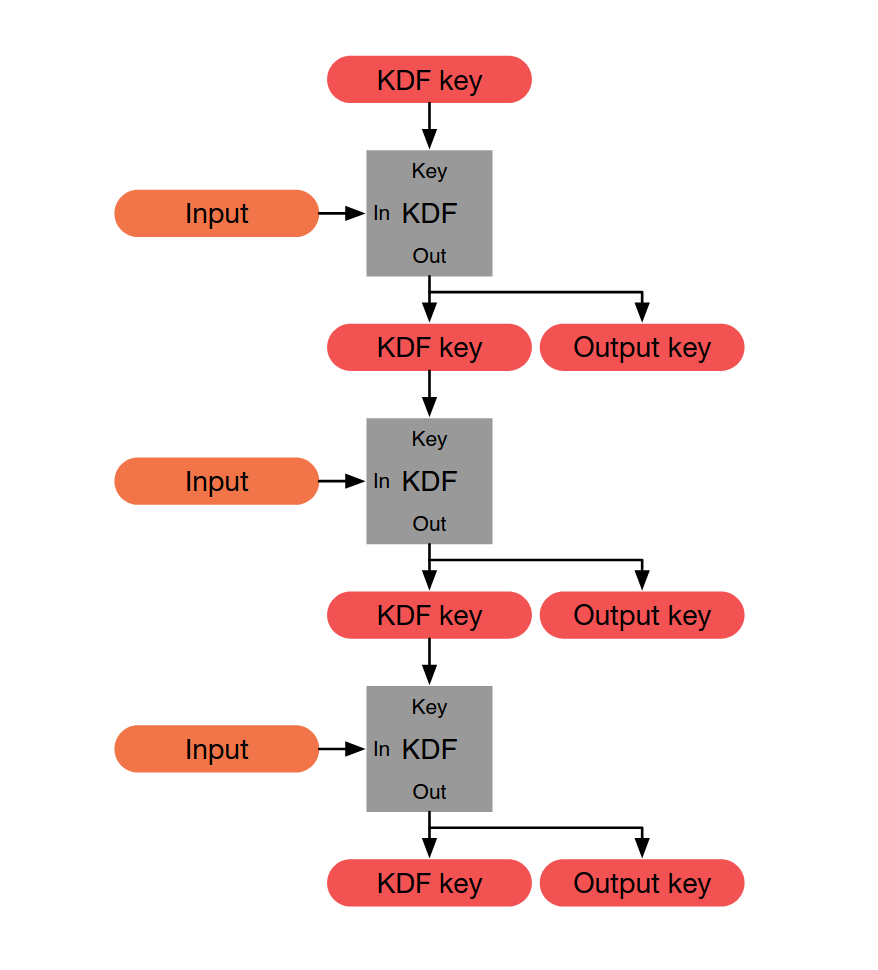
\includegraphics[scale=0.3]{KDF_Chain.png}
  \centering
\end{figure}

A KDF chain has the following properties:

\begin{itemize}
  \item \textbf{Resilience:} The output keys appear random to an adversary without knowledge of the KDF keys. This is true even if the adversary can control the KDF inputs.
  \item \textbf{Forward security:} Output keys from the past appear random to an adversary who learns the KDF key at some point in time.
  \item \textbf{Break-in recovery:} Future output keys appear random to an adversary who learns the KDF key at some point in time, provided that future inputs have added sufficient entropy.
\end{itemize}

In a \textbf{Double ratchet session} between Alice and Bob each party stores a KDF key for three chains: a \textbf{root chain}, a \textbf{sending chain}, and a \textbf{receiving chain}.

As Alice and Bob exchange messages they also exchange new Diffie-Hellman public keys, and the Diffie-Hellman output secretes become the inputs to the root chain. The output keys from the root chain become new KDF keys for the sending and receiving chains. This is called the \textbf{Diffie-Hellman ratchet}.

The sending and receiving chains advanced as each message is sent and received. Their output keys are used to encrypt and decrypt messages. This is called the \textbf{symmetric-key ratchet}.

\subsection{Symmetric-key ratchet}
\label{subsec: Symmetric-keyRatchet}

Every message sent or received is encrypted with a unique \textbf{message key}. The message keys are output keys from the sending and receiving KDF chains. The KDF keys for these chains will be called \textbf{chain keys}.

The KDF inputs for the sending and receiving chains are constant, so these chains don't provide break-in recovery. The sending and receiving chains just ensure that each message is encrypted with a unique key that can be deleted after encryption or decryption. Calculating the next chain key and message key from a given chain key is a single \textbf{ratchet step} in the \textbf{symmetric-key ratchet}.

Since message keys are not used to derive any other keys, message keys may be stored without affecting the security of other message keys. This property is useful for handling lost or out of order messages.

\subsection{Diffie-Hellman ratchet}
\label{subsec:Diffie-HellmanRatchet}

If an attacker steals on party's sending and receiving chain keys, the attacker can compute and decrypt all future messages. To prevent this, the Double Ratchet combines the symmetric-key ratchet with a \textbf{DH ratchet} which updates chain keys based on Diffie-Hellman outputs.

To implement the DH ratchet, each party generates a DH key pair which becomes their current \textbf{ratchet key pair}. Every message from either party begins with a header which contains the sender's current ratchet public key. When a new ratchet public key is received from the remote party, a \textbf{DH ratchet step} is performed which replaces the local party's current ratchet key pair with a new key pair.

This results in a "ping-pong" behavior as the parties take turns replacing ratchet key pairs. An eavesdropper who briefly compromises one of the parties might learn that value of a current ratchet private key, but that private key will eventually be replaced with an uncompromised one. A that point, the Diffie-Hellman calculation between ratchet key pairs will define a DH output unknown to the attacker.

\newpage

\begin{figure}[ht!]
  \centering
  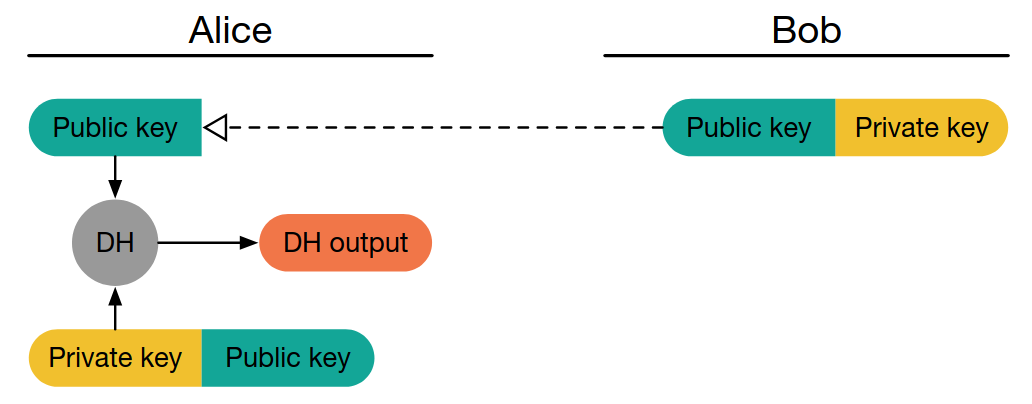
\includegraphics[scale=0.25]{dr1.png}
  \caption{}
  \label{fig:dr1}
\end{figure}

Alice is initialized with Bob's ratchet public key. Alice's ratchet public key isn't yet known to Bob. A part of initialization Alice perform a DH calculation between her ratchet private key and Bob's ratchet public key as shown in figure \ref{fig:dr1}

\begin{figure}[ht!]
  \centering
  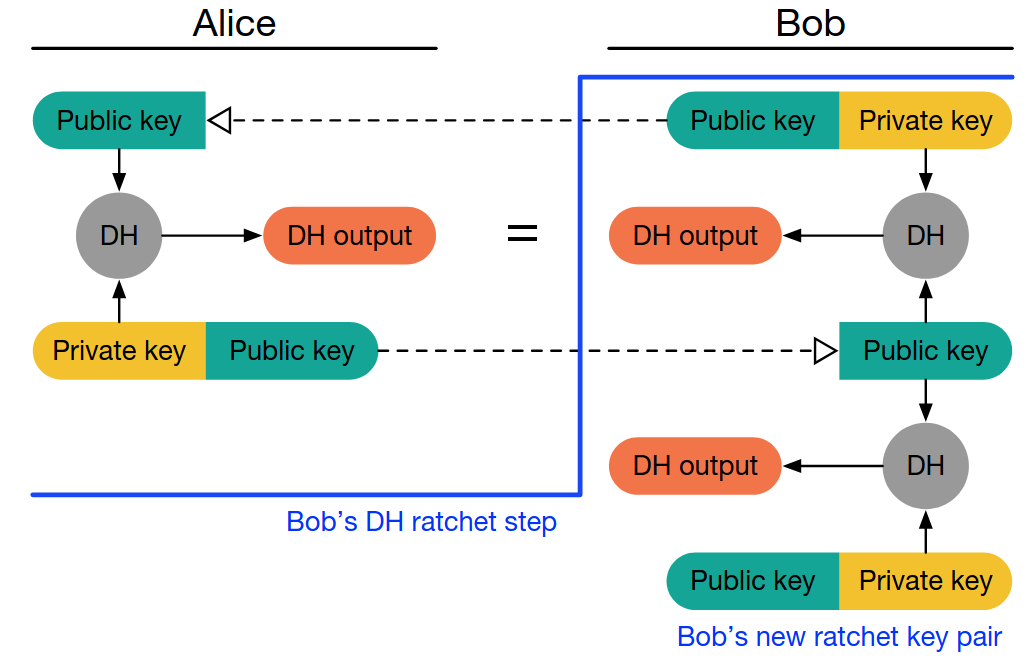
\includegraphics[scale=0.25]{dr2.png}
  \caption{Bob's calculates his DH ratchet step}
  \label{fig:dr2}
\end{figure}

Alice's initial messages advertise her ratchet public key. Once Bob receives one of these messages, Bob performs a DH ratchet step: he calculates the DH output between Alice's ratchet public key and his ratchet private key, which equals Alice's initial DH output. Bob then replaces his ratchet key pair and calculates a new DH output like in figure \ref{fig:dr2}

\newpage

\begin{figure}[ht!]
  \centering
  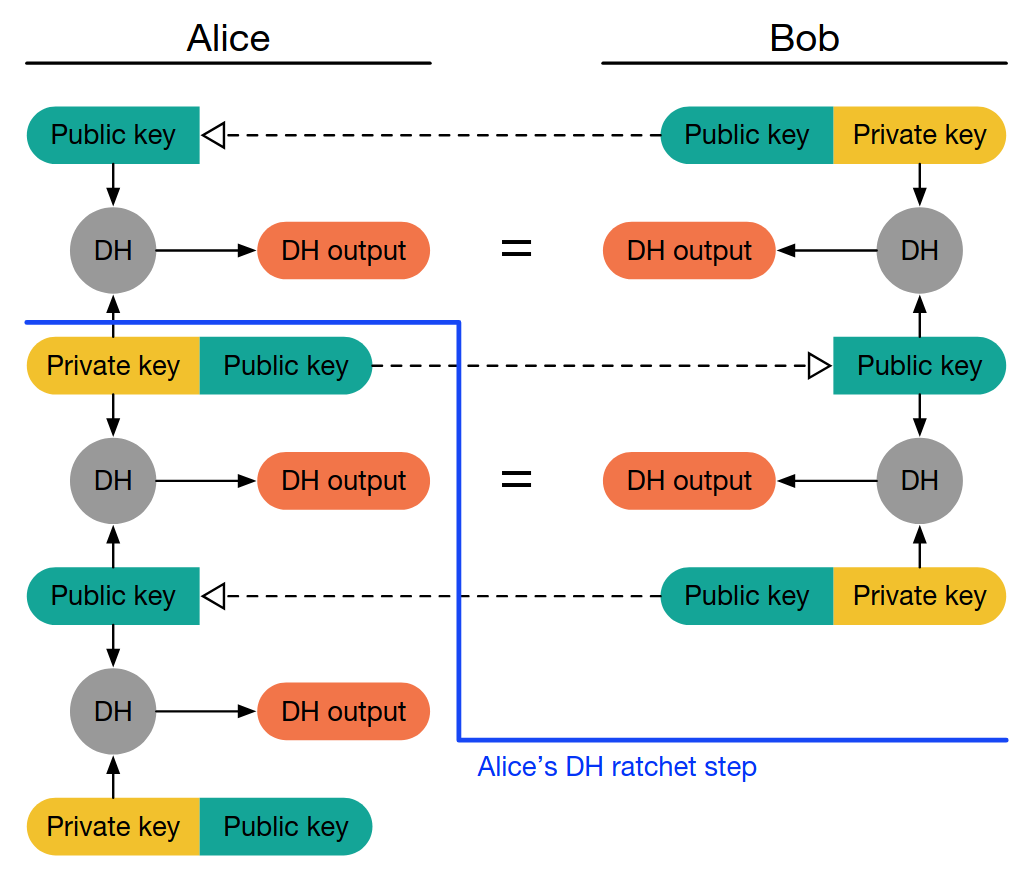
\includegraphics[scale=0.2]{dr3.png}
  \caption{}
  \label{fig:dr3}
\end{figure}

Messages sent by Bob Advertise his new public key. Eventually, Alice will receive one of Bob's messages and perform a DH ratchet step, replacing her ratchet key pair and deriving tow DH outputs, one that matches Bob's latest and a new one \ref{fig:dr3}

\begin{figure}[ht!]
  \centering
  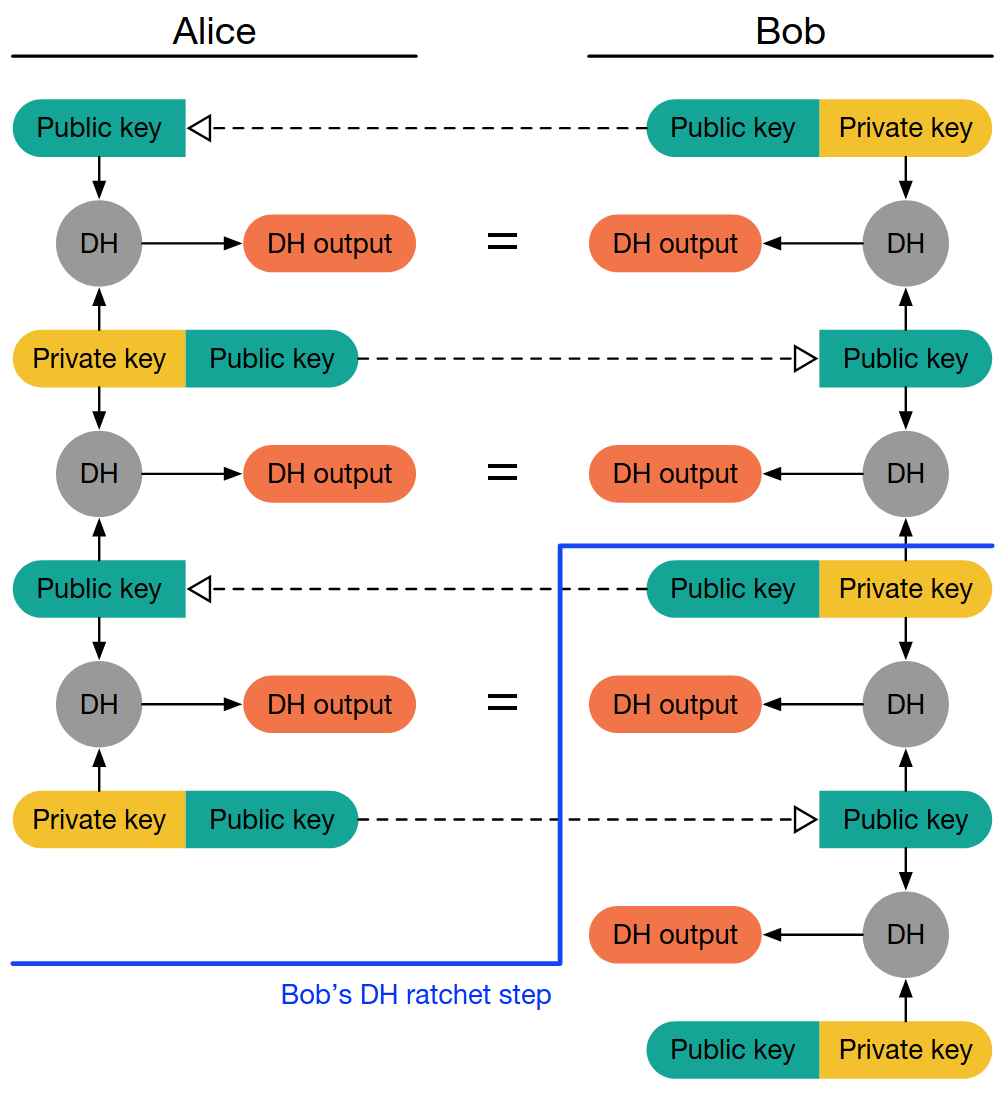
\includegraphics[scale=0.2]{dr4.png}
  \caption{}
  \label{fig:dr4}
\end{figure}

Messages sent by Alice advertise her new public key. Eventually, Bob will receive one of these messages and perform a second DH ratchet step, and so on \ref{fig:dr4}

The DH outputs generated during each DH ratchet step are used to derive new sending and receiving keys. Bob uses his first DH output to derive a receiving chain that matches Alice's sending chain. Bob uses the second DH output to derive a new sending chain. As the parties take turns performing DH ratchet steps, they take turns introducing new sending chains.

However, instead unlike the simplified pictures shown above instead of taking the chain keys directly from DH outputs, the DH outputs are used as KDF inputs to a root chain, and the KDF outputs from the root chain are used as sending and receiving chain keys. Using a KDF chain here improves resilience and break-in recovery. A full DH ratchet step consists of updating the root KDF chain twice, and using the KDF output keys as new receiving and sending chain keys:

\begin{figure}[ht!]
  \centering
  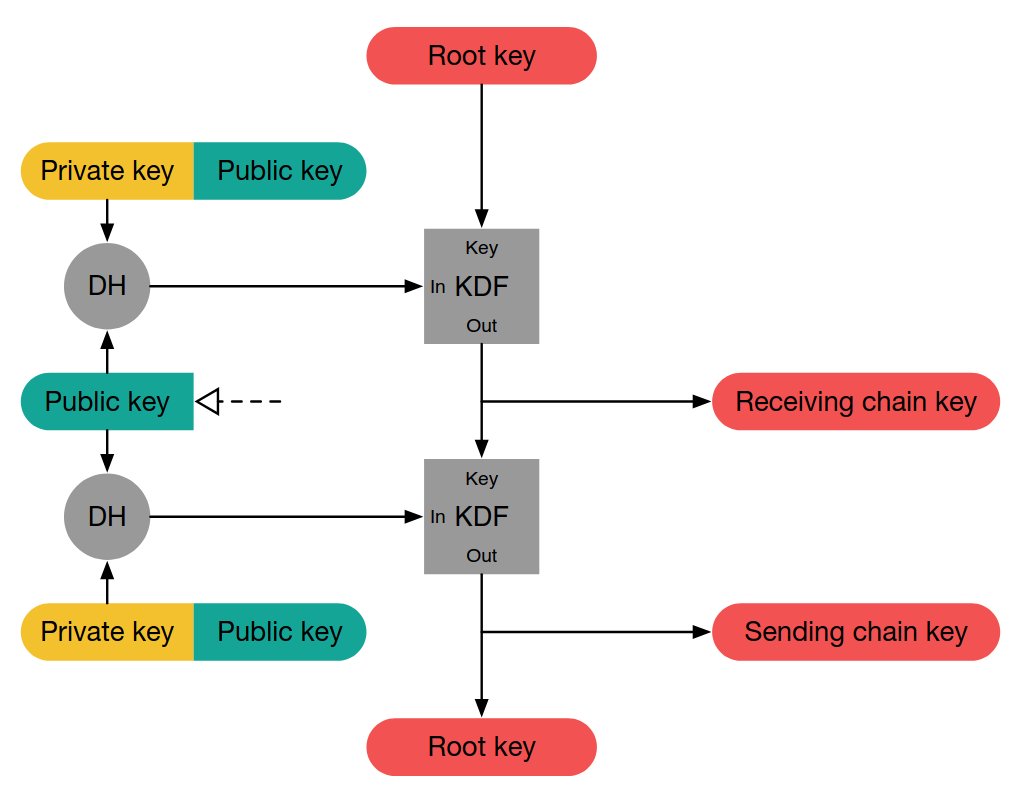
\includegraphics[scale=0.3]{dr5.png}
  \caption{}
  \label{fig:dr5}
\end{figure}

\subsection{Combining both Ratchets}
\label{subsec:CombiningBothRatchets}

Combining the symmetric-key and DH ratchets gives the Double Ratchet:

\begin{itemize}
  \item When a message is sent or received, a symmetric-key ratchet step is applied to the sending or receiving chain to derive the message key.
  \item When a new ratchet public key is received a DH ratchet step is per formed prior to the symmetric-key ratchet to replace the chain keys.
\end{itemize}

In figure \ref{fig:dr6} Alice has been initialized with Bob's ratchet public key and a shared secret which is the initial root key. As part of initialization Alice generates a new ratchet key pair, and feeds the DH output to the root KDF to calculate a new root key $(RK)$ and sending chain key $(CK)$:

\begin{figure}[ht!]
  \centering
  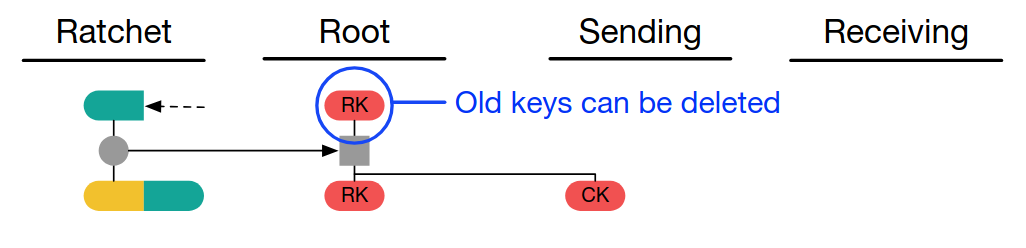
\includegraphics[scale=0.3]{dr6.png}
  \caption{}
  \label{fig:dr6}
\end{figure}

When Alice sends her first message $A1$, she applies a symmetric-key ratchet step to her sending chain key, resulting in a new message key. The new chain key is stored, but the message key and old chain key can be deleted \ref{fig:dr7}

\begin{figure}[ht!]
  \centering
  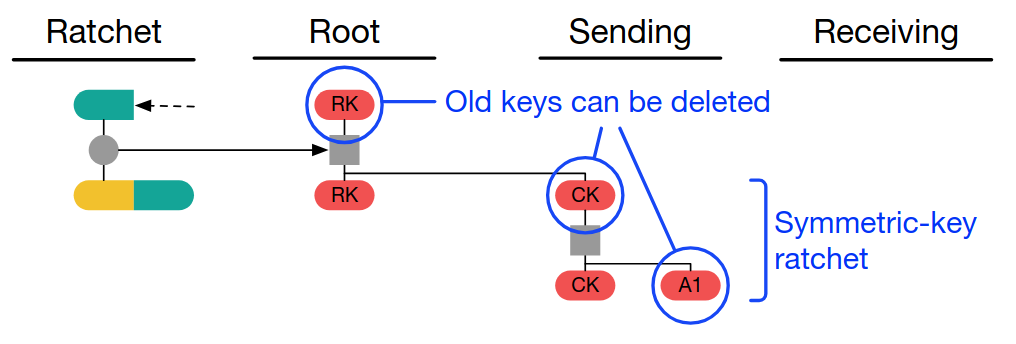
\includegraphics[scale=0.3]{dr7.png}
  \caption{}
  \label{fig:dr7}
\end{figure}

If Alice next receives a response $B1$ from Bob, it will contain a new ratchet public key. Alice applies a DH ratchet step to derive new receiving and sending chain keys. Then she applies a symmetric-key ratchet step to the receiving chain to get the message key for the received message \ref{fig:dr8}

\begin{figure}[ht!]
  \centering
  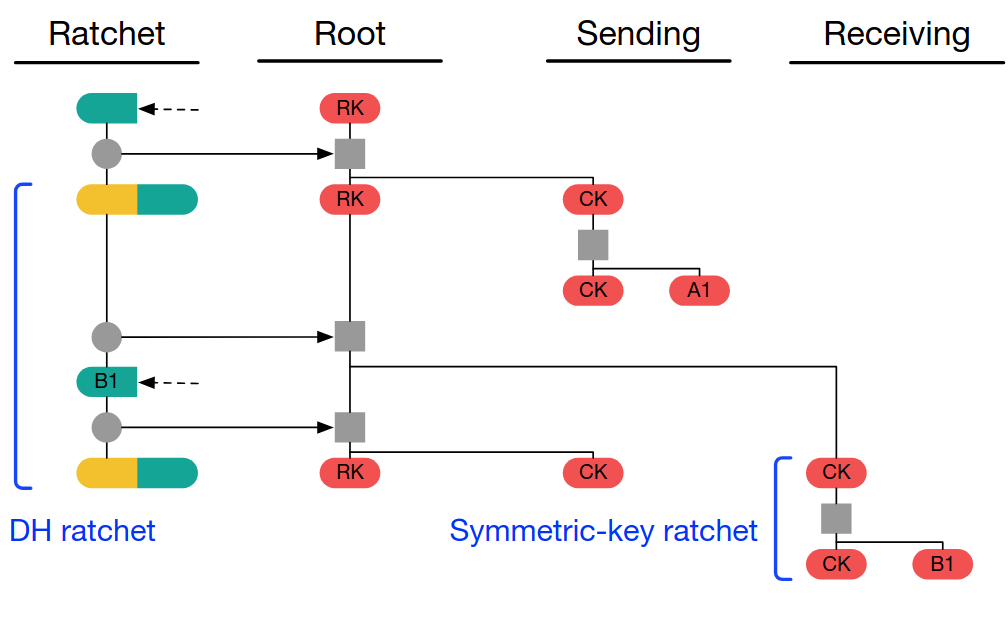
\includegraphics[scale=0.3]{dr8.png}
  \caption{}
  \label{fig:dr8}
\end{figure}

Suppose Alice next sends a message $A2$, receives a message $B2$ with Bob’s old ratchet public key, then sends messages $A3$ and $A4$. Alice’s sending chain will ratchet three steps, and her receiving chain will ratchet once \ref{fig:dr9}

\begin{figure}[ht!]
  \centering
  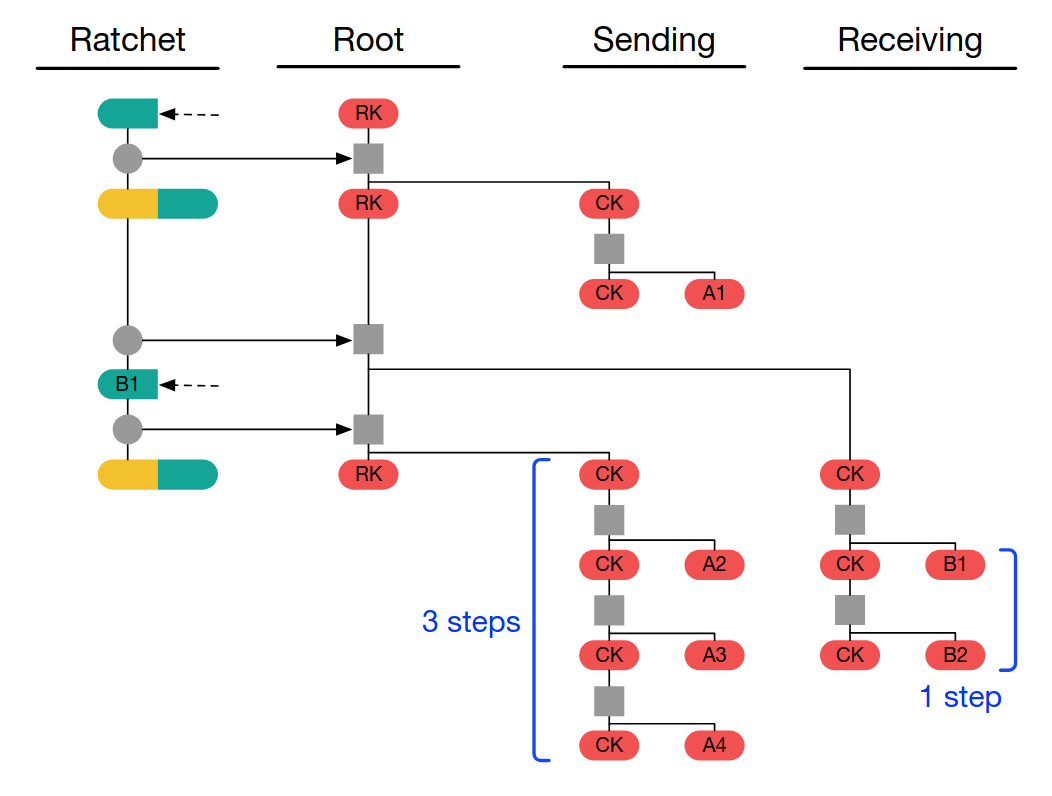
\includegraphics[scale=0.3]{dr9.png}
  \caption{}
  \label{fig:dr9}
\end{figure}

Suppose Alice then receives messages $B3$ and $B4$ with Bob’s next ratchet key, then sends a message $A5$. Alice’s final state will be as follows \ref{fig:dr10}

\begin{figure}[ht!]
  \centering
  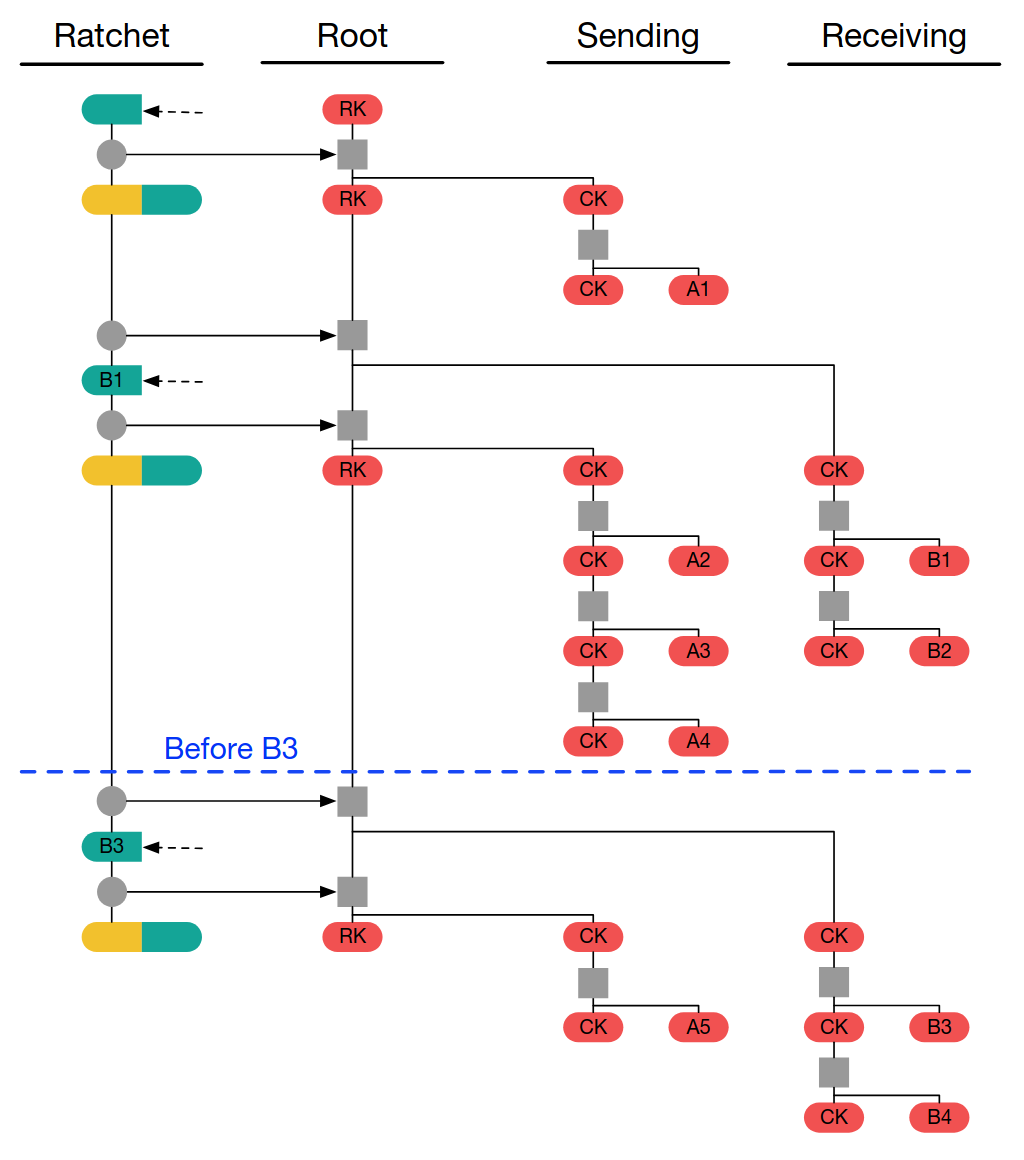
\includegraphics[scale=0.3]{dr10.png}
  \caption{}
  \label{fig:dr10}
\end{figure}

\subsection{Out-of-order messages}
\label{Out-of-orderMessages}

The Double Ratchet handles lost or out-of-order messages by including in each message header the message’s number in the sending chain and the length in the previous sending chain $PN$. This enables the recipient to advance to the relevant message key while storing skipped message keys in case the skipped messages arrive later.

On receiving a message, if a DH ratchet step is triggered then the received $PN$ minus the length of the current receiving chain is the number of skipped messages. The received $N$ is the number of skipped messages in the new receiving chain.

If a DH ratchet step is not triggered, then the received $N$ minus the length of the receiving chain is the number of skipped messages in that chain.

For example, consider the message sequence from the previous section \ref{fig:dr10} when messages $B2$ and $B3$ are skipped. Message $B4$ will trigger Alice’s DH ratchet step (instead of $B3$). Message $B4$ will have $PN = 2$ and $N =1$. On receiving $B4$ Alice will have a receiving chain of length 1 ($B1$), so Alice will store message keys for $B2$ and $B3$, so they can be decrypted if they arrive later as it is shown in figure \ref{fig:dr11}:

\begin{figure}[ht!]
  \centering
  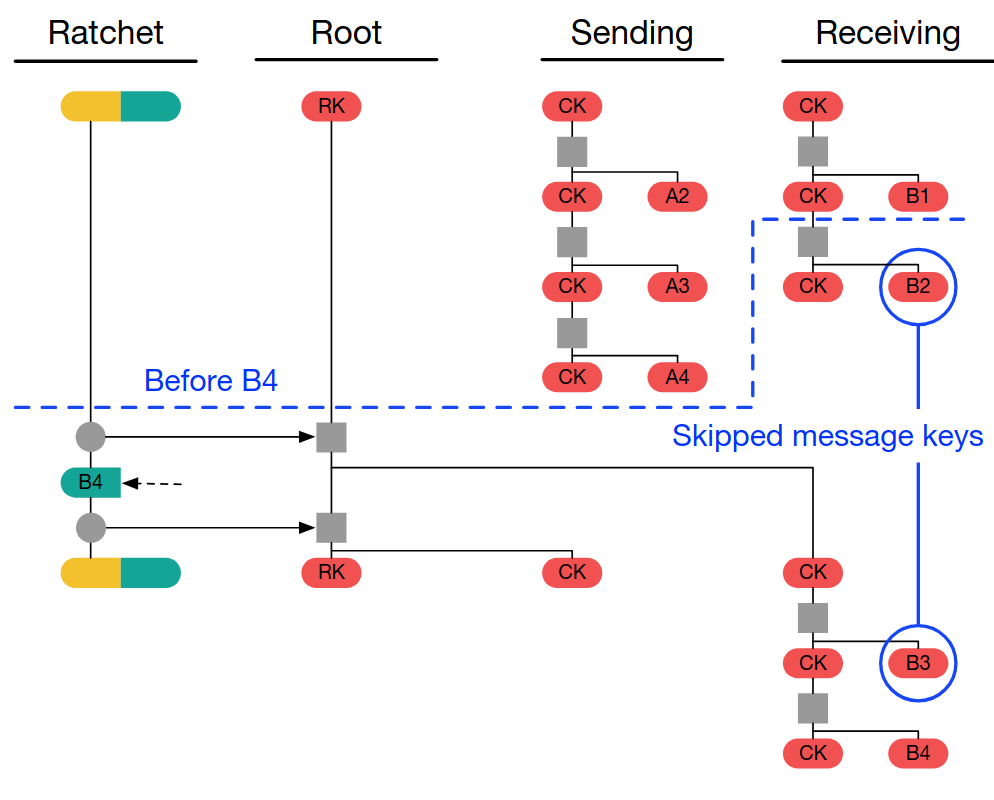
\includegraphics[scale=0.3]{dr11.png}
  \caption{}
  \label{fig:dr11}
\end{figure}

\section{Integration with X3DH}
\label{sec:IntegrationWithX3DH}

The outputs of the X3DH are used by the Double Ratchet:
\begin{itemize}
  \item The $SK$ output from X3DH becomes the $SK$ input to Double ratchet initialization.
  \item The $AD$ output from X3DH becomes the $AD$ input to Double Ratchet encryption and decryption.
  \item Bob's signed prekey form X3DH ($SPK_B$) becomes Bob's initial ratchet public key for double ratchet initialization.
\end{itemize}

\section{Security Considerations}
\label{sec:SecurityConsideration}

\subsection{Authentication}
\label{subsec:Authentication}

Before or after an X3DH key agreement, the parties may compare their identity public keys $IK_A$ and $IK_B$ through some authenticated channel. For example, they may compare public key fingerprints manually, or by scanning a QR code.

During the designing phase of our project we assumed that the server could not be impersonated by any malicious attacker and can not be tampered with thus making sure that what Alice or Bob get from the server are the correct keys.

\subsection{Protocol Replay}
\label{subsec:ProtocolReplay}

One of the potential issues of X3DH is the possibility of a replay attack, but this is no possible thanks to the implementation of the one-time prekys. In Signal's documentation other proposed mitigations are: use a ratchet mechanism, keep a blacklist of observed messages, or replace old signed prekeys more rapidly.

\subsection{Deniability}
\label{subsec:Deniability}

X3DH doesn’t give either Alice or Bob a publishable cryptographic proof of the contents of their communication or the fact that they communicated.

Like in the OTR protocol \cite{OTR}, in some cases a third party that has compromised legitimate private keys from Alice or Bob could be provided a communication transcript that appears to be between Alice and Bob and that can only have been created by some other party that also has access to legitimate private keys from Alice or Bob.

\subsection{Key Compromise}
\label{subsec:KeyCompromise}

Compromise of a party's private keys has a huge impact on security, though the use of ephemeral keys and prekeys provides some mitigation.

Compromise of a party's identity private key allows impersonation of that party to others. Knowledge of a party's preky private keys may affect the security of older or newer $SK$ values, depending on many factors.

Since we implemented one-time prekeys then the compromise of identity keys and preky private keys at some future time will not compromise older $SK$ since the $OPK_B$ was deleted. Moreover, we also implemented double ratchet which replaces $SK$ with new keys to provide fresh forward secrecy.

\subsection{Server Trust}
\label{subsec:ServerTrust}

A malicious server could cause communication between Alice and Bob to fail for example by refusing to deliver messages.

The other possible issue is the inability to check in person keys, but a system similar to the one implemented by many Linux distros should suffice as integrity check for the key of the server. Once we have established a root of trust we can rely on the checks implemented by the protocol.

Another final possible attack is due to the limited number of $OTK$ if an attacker drains another party's one-time prekys, making them unable to create new connections. A system to replenish one-time prekys should be implemented, and the server should limit the rate keys are requested.

\subsection{Secure Deletion}
\label{subsec:SecureDeletion}

The double ratchet algorithm is designed to provide security against and attacker who records encrypted messages and then compromises the sender or receiver at a later time. This security could be deleted if deleted plaintext or keys could be recovered by an attacker with low-level access to the compromised device. But the main focus of this project is security of data in transit.

\subsection{Recovery from Compromise}
\label{subsec:RecoveryFromCompromise}

The DH ratchet is designed to recover security against a passive eavesdropper who observes encrypted messages after compromising the parties to a session. Compromise of secrete keys will:

\begin{itemize}
  \item The attacker could use the compromised keys to impersonate the compromised party.
  \item The attacker could substitute her own ratchet keys via continuous active MitM attack, to maintain eavesdropper on the compromised session.
  \item The attacker could modify a compromised party's RNG so that future ratchet private keys are predictable.
\end{itemize}

If a party suspects its keys or devices have been compromised, it must replace them immediately.

\subsection{Cryptanalysis and Ratchet Public Keys}
\label{subsec:CryptanalysisandRatchetPublicKeys}

Because all DH ratchet computations are mixed into the root key, an attacker who can decrypt a session with passive cryptanalysis, an attacker who can decrypt a session with passive cryptanalysis might lose this ability if she fails to observe some ratchet public keys.

But in our implementation cryptanalysis should not be an issue due to the use of strong encryption function like AES-GCM.

\subsection{Deletion of Skipped Message Keys}
\label{subsec:DeletionofSkippedMessageKeys}

Storing skipped message keys introduces some risks:

\begin{itemize}
  \item A malicious sender could induce recipients to store large numbers of skipped message keys, possibly causing DoS due to consuming storage space.
  \item The lost messages may have been seen by an attacker, even though they did not reach the recipient. The attacker can compromise the intended recipient at a later time to retrieve the skipped message keys.
\end{itemize}

The implemented mitigation is limiting the number of skipped messages to 1000. For the second one we created a set timer after which keys are deleted as proposed by the Signal documentation.
